\chapter{Introduction}
\section{Background: energy storage}
The demand for ever improving energy storage solutions is driven by both commercial interests and an urgent societal need.
In order to curtail \ce{CO2} emissions and limit the impact of global warming, a shift from fossil-fuel based energy generation towards renewable energy is vital.\cite{Goodenough2013}
Unfortunately, a characteristic of many renewable energy sources, such as wind and solar energy, is the intermittent nature of its generation, \cite{Goodenough2010a,Ellis2012,Liu2013} requiring energy storage solutions.

Vehicle electrification may displace conventional combustion engine driven transport, another major source of greenhouse gases and pollution.\cite{Blomgren2017}
While some commercial success has being enjoyed by electric vehicles in recent years, concerns surrounding safety, longevity, and insufficient energy density to overcome ``range anxiety'' demands further development of battery materials and technologies for widespread adoption of electric vehicles to occur.\cite{Cano2018a,Schmuch2018}

In addition, consumer demand for increasingly powerful, thin, and light portable electronics with larger times between charges has pushed current battery chemistries to their limits.\cite{Liu2010}
With the majority of developments in batteries for portable electronics in recent years arising not from improvements in their chemistries, but by improved manufacturing processes with diminishing returns, the need for a fundamentally different battery may arise in the near future.
Indeed, in recent years a number of manufacturers have, in a drive to yield more performance from the same materials, produced cells which ultimately proved to be unsafe.\cite{Loveridge2018}
Any given application will prioritise different properties in their energy storage solutions, requiring different battery materials to be developed and improved upon.

\section{Li-ion batteries}
Lithium, being the lightest and most electropositive metal,\cite{Tarascon2010} is well suited to applications in high density energy storage.
The first commercial Li-ion battery was developed in the 1980's by John Goodenough\cite{Mizushima1981} and manufactured by Sony Co. in 1991.\cite{Li2018}
This development, coupled with the rapid decrease in the size of transistors, sparked the portable electronics revolution.
In the years since, a range of battery chemistries have been developed, tailored to specific applications.

\subsection{Anatomy of an electrochemical cell}
Figure \ref{fig:Goodenough} illustrates a typical electrochemical cell, specifically the first commercial Li-ion battery.
The cell consists of an anode and cathode which are electrically isolated from one another, but able to freely exchange ions via an electrolyte.
The cell is charged by applying an external potential across the cell, forcing electrons to the anode.
\ce{Li+} ions are extracted from the \ce{LiCoO2} cathode, diffuse between the electrodes via an electrolyte (\ce{LiFP6 in organic solvent} typically), and intercalate into the anode structure to maintain charge neutrality.

During discharge, the reverse process occurs.
\ce{Li+} ions driven by a difference in chemical potential move from the anode to the cathode, and electrons travel via an external circuit to maintain charge neutrality, allowing useful work to be done.


\begin{figure}
\centering
\begin{subfigure}{\linewidth}
  \centering
  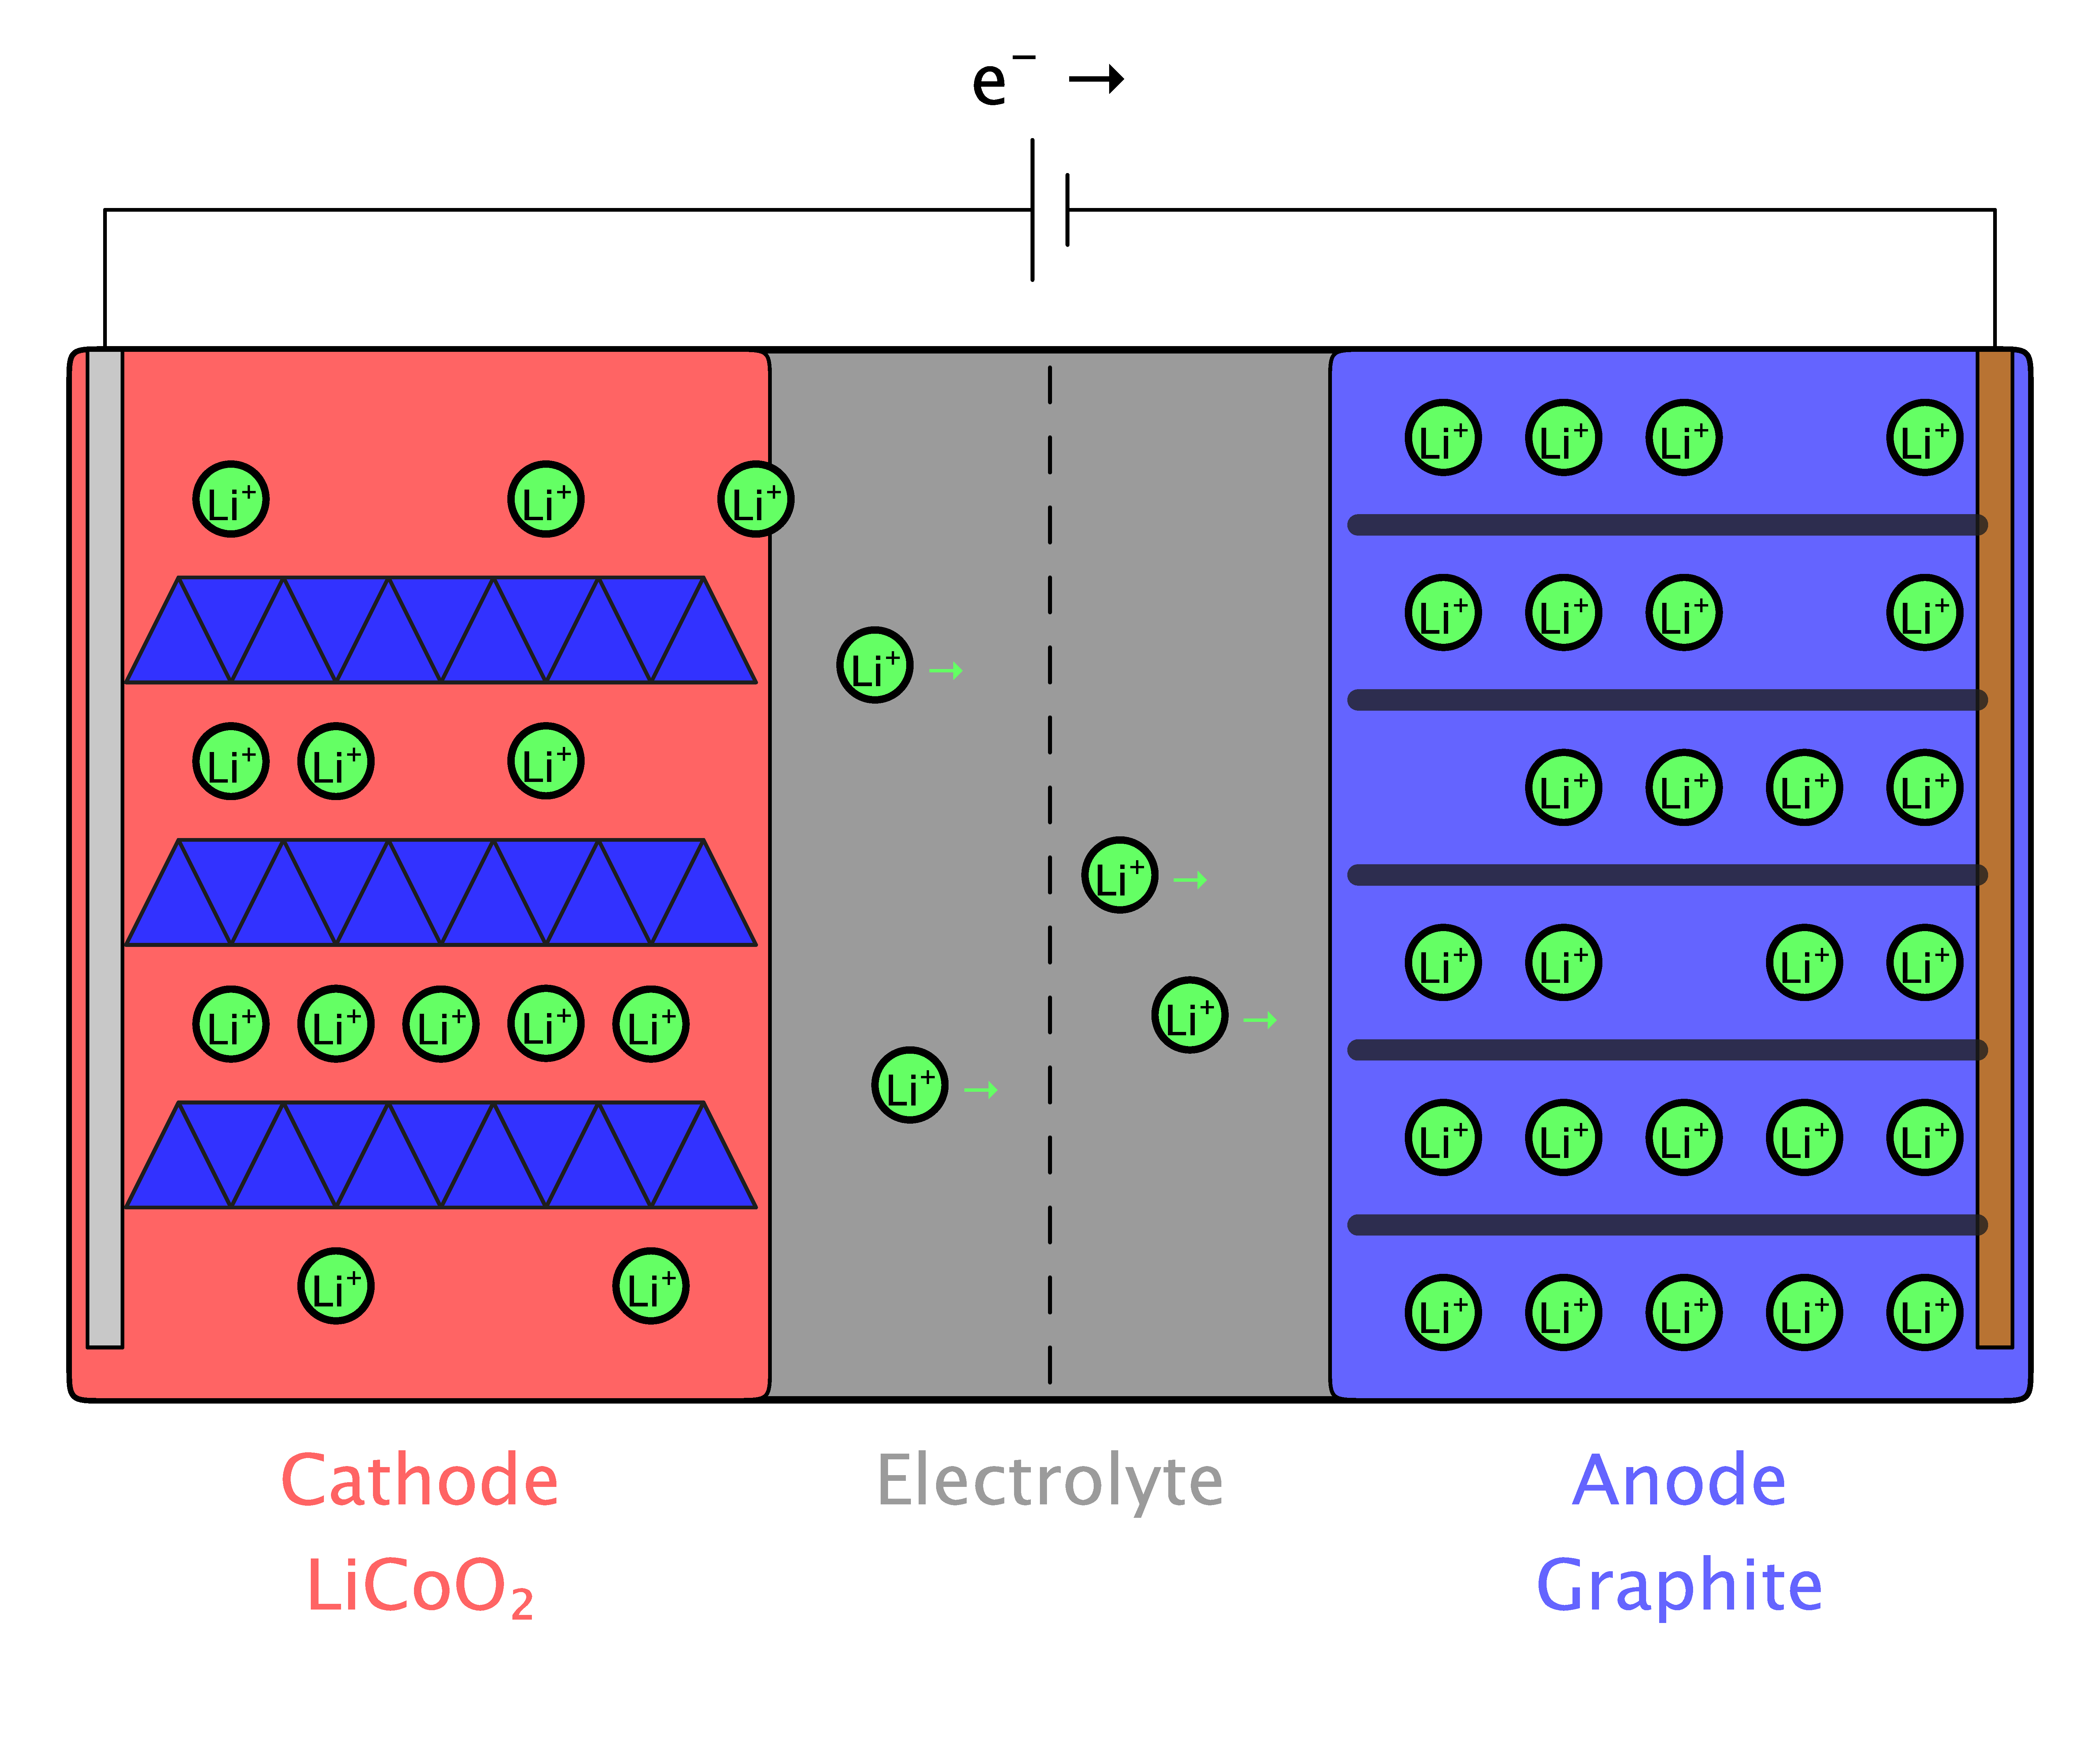
\includegraphics[width=0.7\linewidth, trim=1cm 1cm 1cm 1cm, clip]{figures/batteryCharge/batteryCharge}
  \caption{Charging}
  \label{fig:GoodenoughCharging}
\end{subfigure}

\begin{subfigure}{\linewidth}
  \centering
  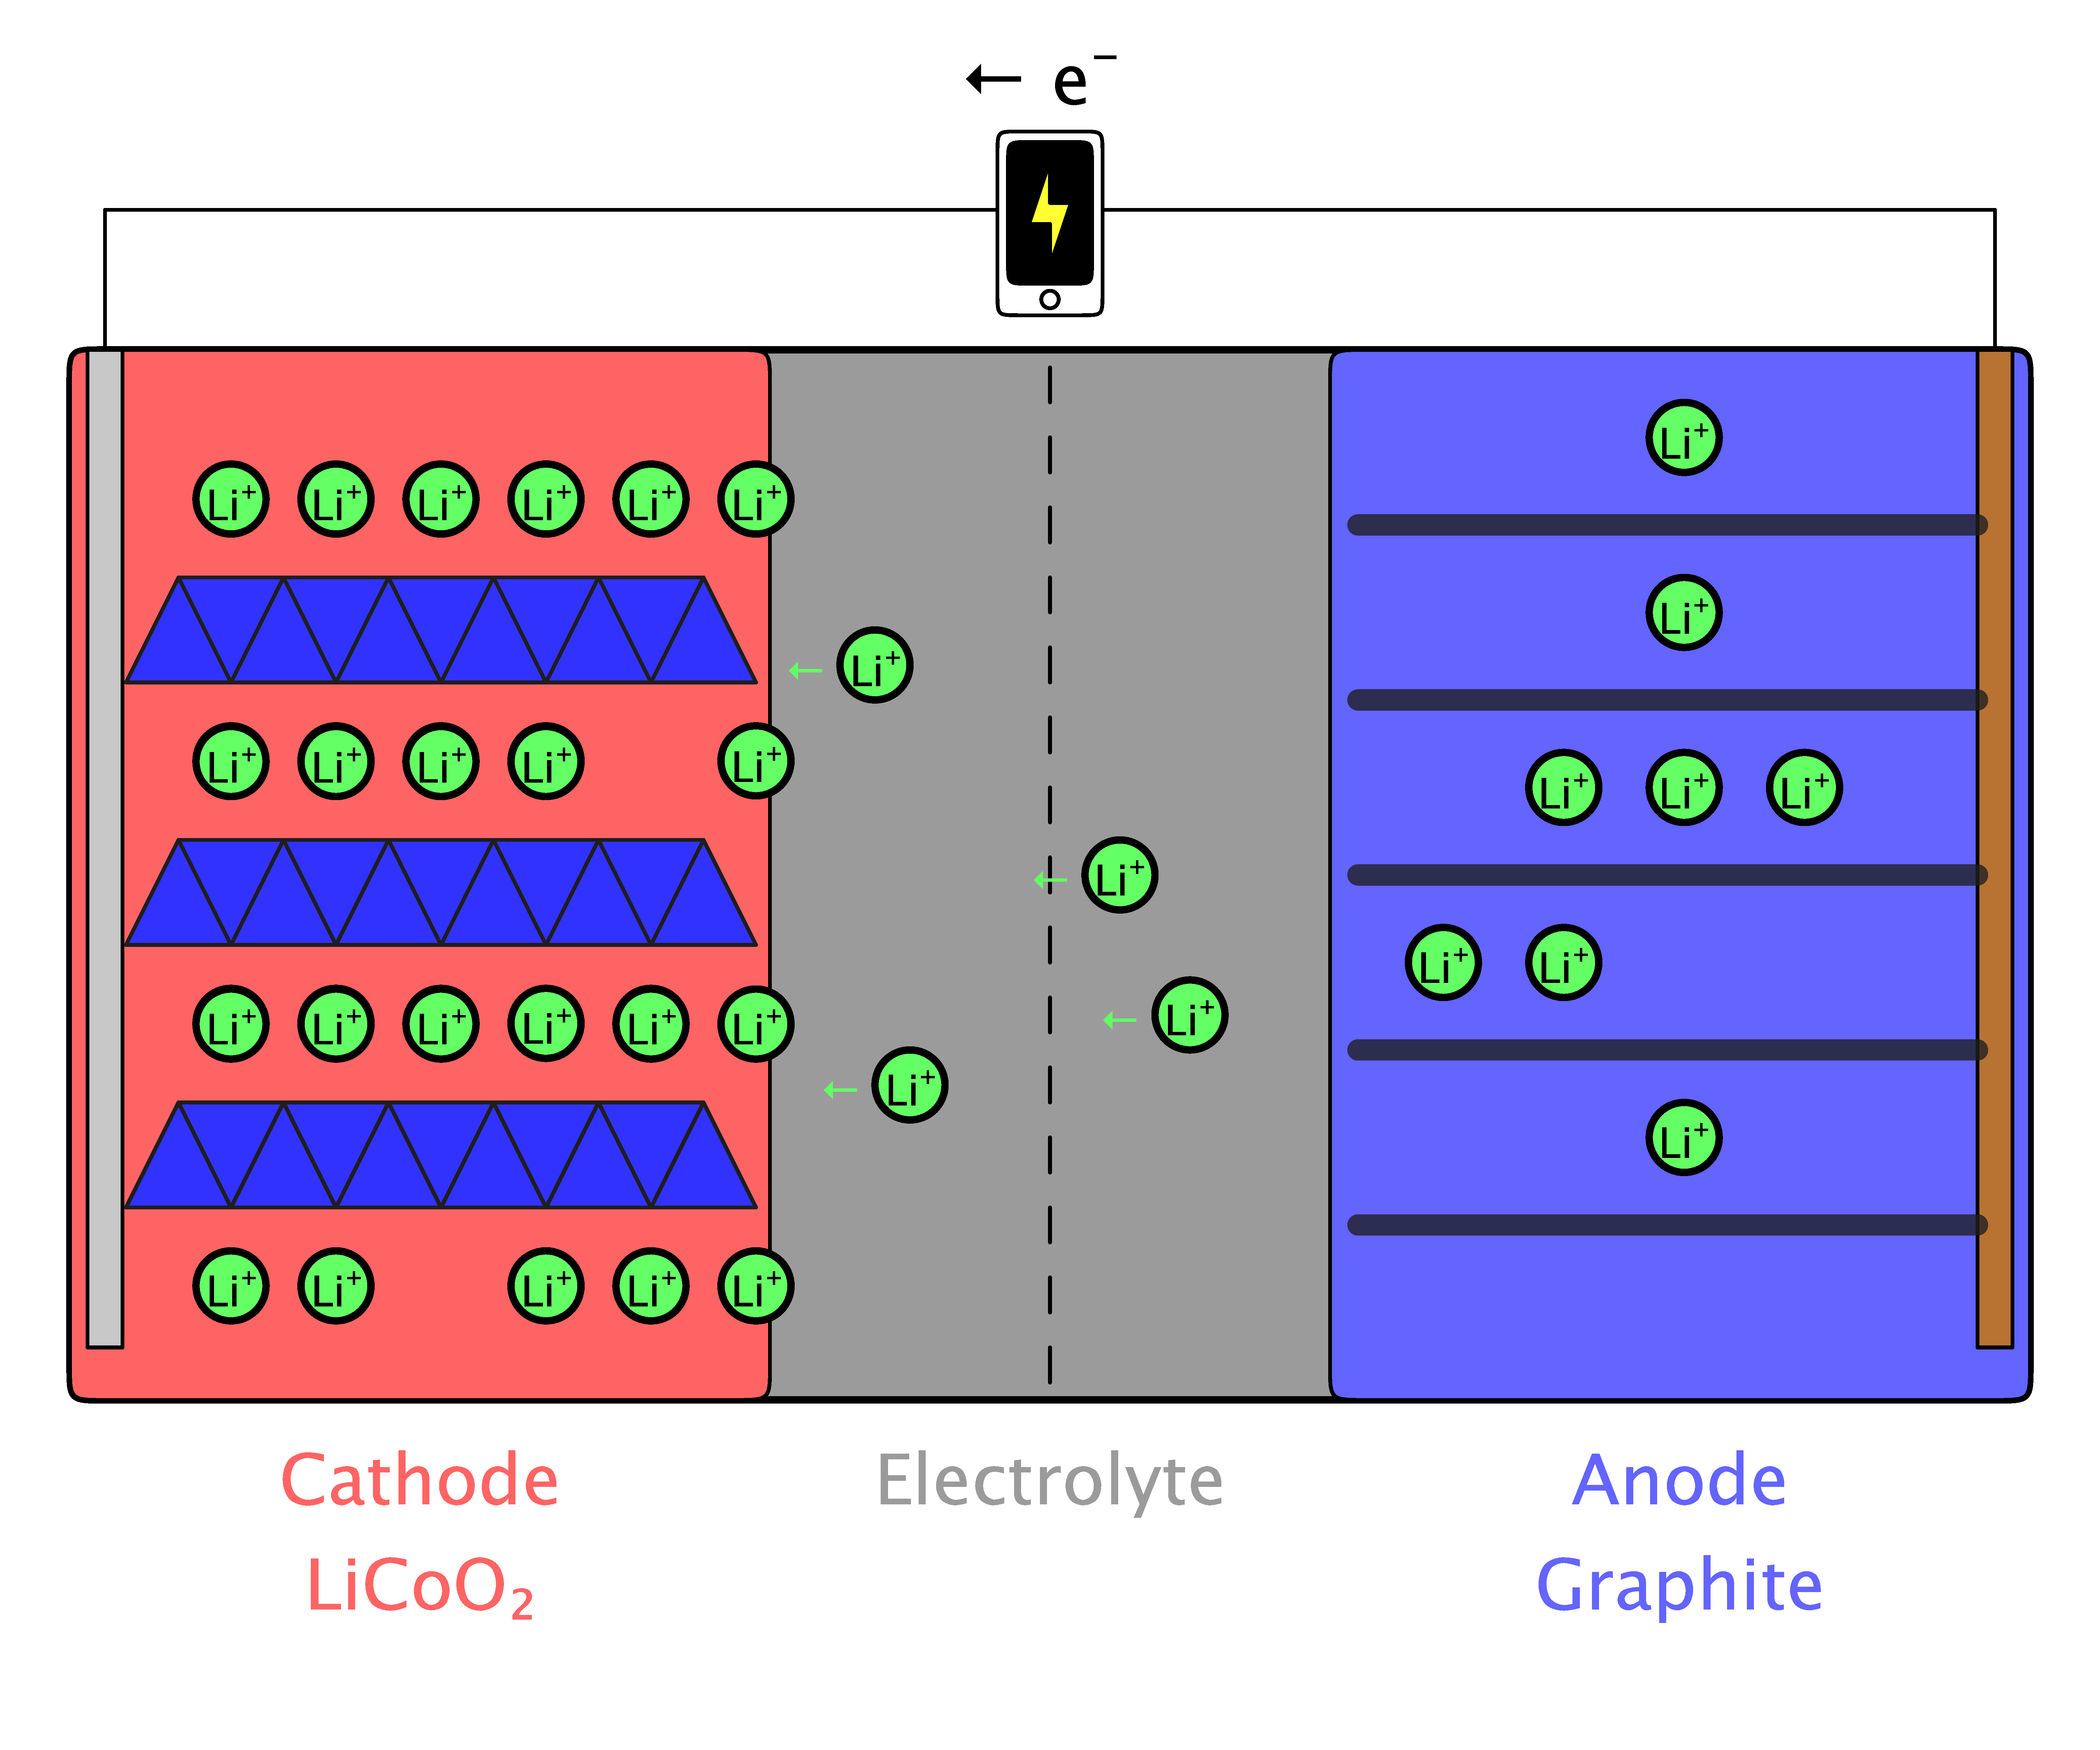
\includegraphics[width=0.7\linewidth, trim=1cm 1cm 1cm 1cm, clip]{figures/batteryDischarge/batteryDischarge}
  \caption{Discharging}
  \label{fig:GoodenoughDischarging}
\end{subfigure}
\caption[Li-ion battery schematic]{A schematic of a common Li-ion battery. During charging (a), electrons are driven to the anode by an external potential. \ce{Li+} ions move from the cathode to the anode to maintain charge neutrality. During discharge (b), \ce{Li+} ions are driven to the cathode by a difference in chemical potential. As the electrodes are electrically isolated from one another by the separator, electrons are instead forced to travel via an external circuit and provide work.} 
\label{fig:Goodenough}
\end{figure}

\newpage
\section{Electrolyte materials}
In order for useful work to be yielded from batteries, and in order to prevent short circuiting, the electrodes must be electrically isolated from one another.\cite{Palacin2009}
In practice, this is implemented by use of a porous but electrically insulating separator material (typically a multilayer polymer) coupled with an electrolyte material.
As the rate at which the battery can discharge is dependant on the rate at which the electrodes can exchange \ce{Li+} ions, high ionic conductivity is vital for commercially viable electrolytes.


\subsection{Liquid electrolytes}
All Li-ion battery systems currently available commercially use liquid electrolytes.\cite{Famprikis2019}
These typically consist of \ce{LiFP6} salts dissolved in a mixture of organic solvents.
The exact composition will vary dependant on the choice of electrodes, application, and manufacturer.
That said, the use of ethyl methyl carbonate (EC) is universal in organic electrolytes, as its inclusion results in the formation of a passivating layer on graphite anodes, preventing solvent molecules from intercalating into the anode and destroying the graphitic structure.\cite{Palacin2009}

These electrolyte solutions are typically stable to \SI{3.5}{\volt}, above which the electrolyte decomposes in a kinetically limited process.
As conventional batteries are often charged above \SI{3.5}{\volt}, this causes a slow decline in the performance of the battery over time.
The use of hierarchical electrode materials may mitigate this issue and allow the use of higher voltage cathode chemistries. \cite{Zhou2018}

\subsection{Solid electrolytes}
Solid-state batteries have been of significant research interest in recent years, primarily due to the increased safety they can offer.\cite{Famprikis2019, Zhang2018, Manthiram2017a, Janek2016}
Liquid electrolytes typically consist of highly flammable organic solvents which lead to dangerous failure modes.
The use of such electrolytes in EV applications, where mechanical failure of batteries is likely in the event of a crash, can significantly enhance the safety of EV's.

They can also offer higher energy densities, by enabling the use of higher energy density electrode materials which cannot be in liquid electrolyte systems.
In particular, they may allow the use of Li-metal anodes (see Section \ref{sec:anodes}), increasing the energy density of the anode by an order of magnitude,\cite{Zhang2018} and high voltage cathode materials for which no known stable liquid electrolyte exists.

\section{Anode materials}
\label{sec:anodes}
Li metal is theoretically the best possible anode material with a huge theoretical capacity (\SI{3860}{\milli\ampere\hour\per\gram}/\SI{2061}{\milli\ampere\hour\per\centi\meter\cubed}), and was used in early Li battery research. 
Unfortunately, dendrite formation at the anode surface ultimately leads to short circuiting and fires, preventing its use with current commercially viable electrolytes. \cite{Cheng2017,Guo2017a,Lin2017,Placke2017}
As such, current commercial batteries generally use a graphitic anode which undergoes the following reversible reaction:\cite{Islam2014}
\begin{equation}
\ce{Li_xC6(s) <-> $x$Li+(soln) +6C(s) + $x$e-}
\end{equation}
The performance of graphite anodes is a function of their morphology,\cite{Buqa2005} meaning the capacity achieved is strongly influenced by the manufacturing processes used and the state of health of the battery.

The use of graphite (albeit value-added graphite) as a key material in batteries is of course a huge advantage due to its high abundance, low cost, and excellent electrical conductivity.
Whilst the graphite anodes are not the current limiting factor in commercial batteries, having higher capacities (\SI{372}{\milli\ampere\hour\per\gram}) than the best available cathodes, they are still of research interest in anticipation of next-generation cathodes.

Tin and silicon based alloys offer higher capacities than graphite, but are currently not viable due to myriad issues including large volume changes (+200\% for Si) over a charge/discharge cycle.\cite{Scrosati2011}

\newpage
\section{Cathode materials}
Cathode materials are currently the limiting factor in commercial batteries, making them a highly active and rapidly changing field of research.\cite{Marom2011}
While a wide range of materials are currently of research interest, only a few classes of cathode materials have enjoyed widespread commercialisation thus far.

\subsection{\ce{LiMO2}}
\begin{figure}
\centering
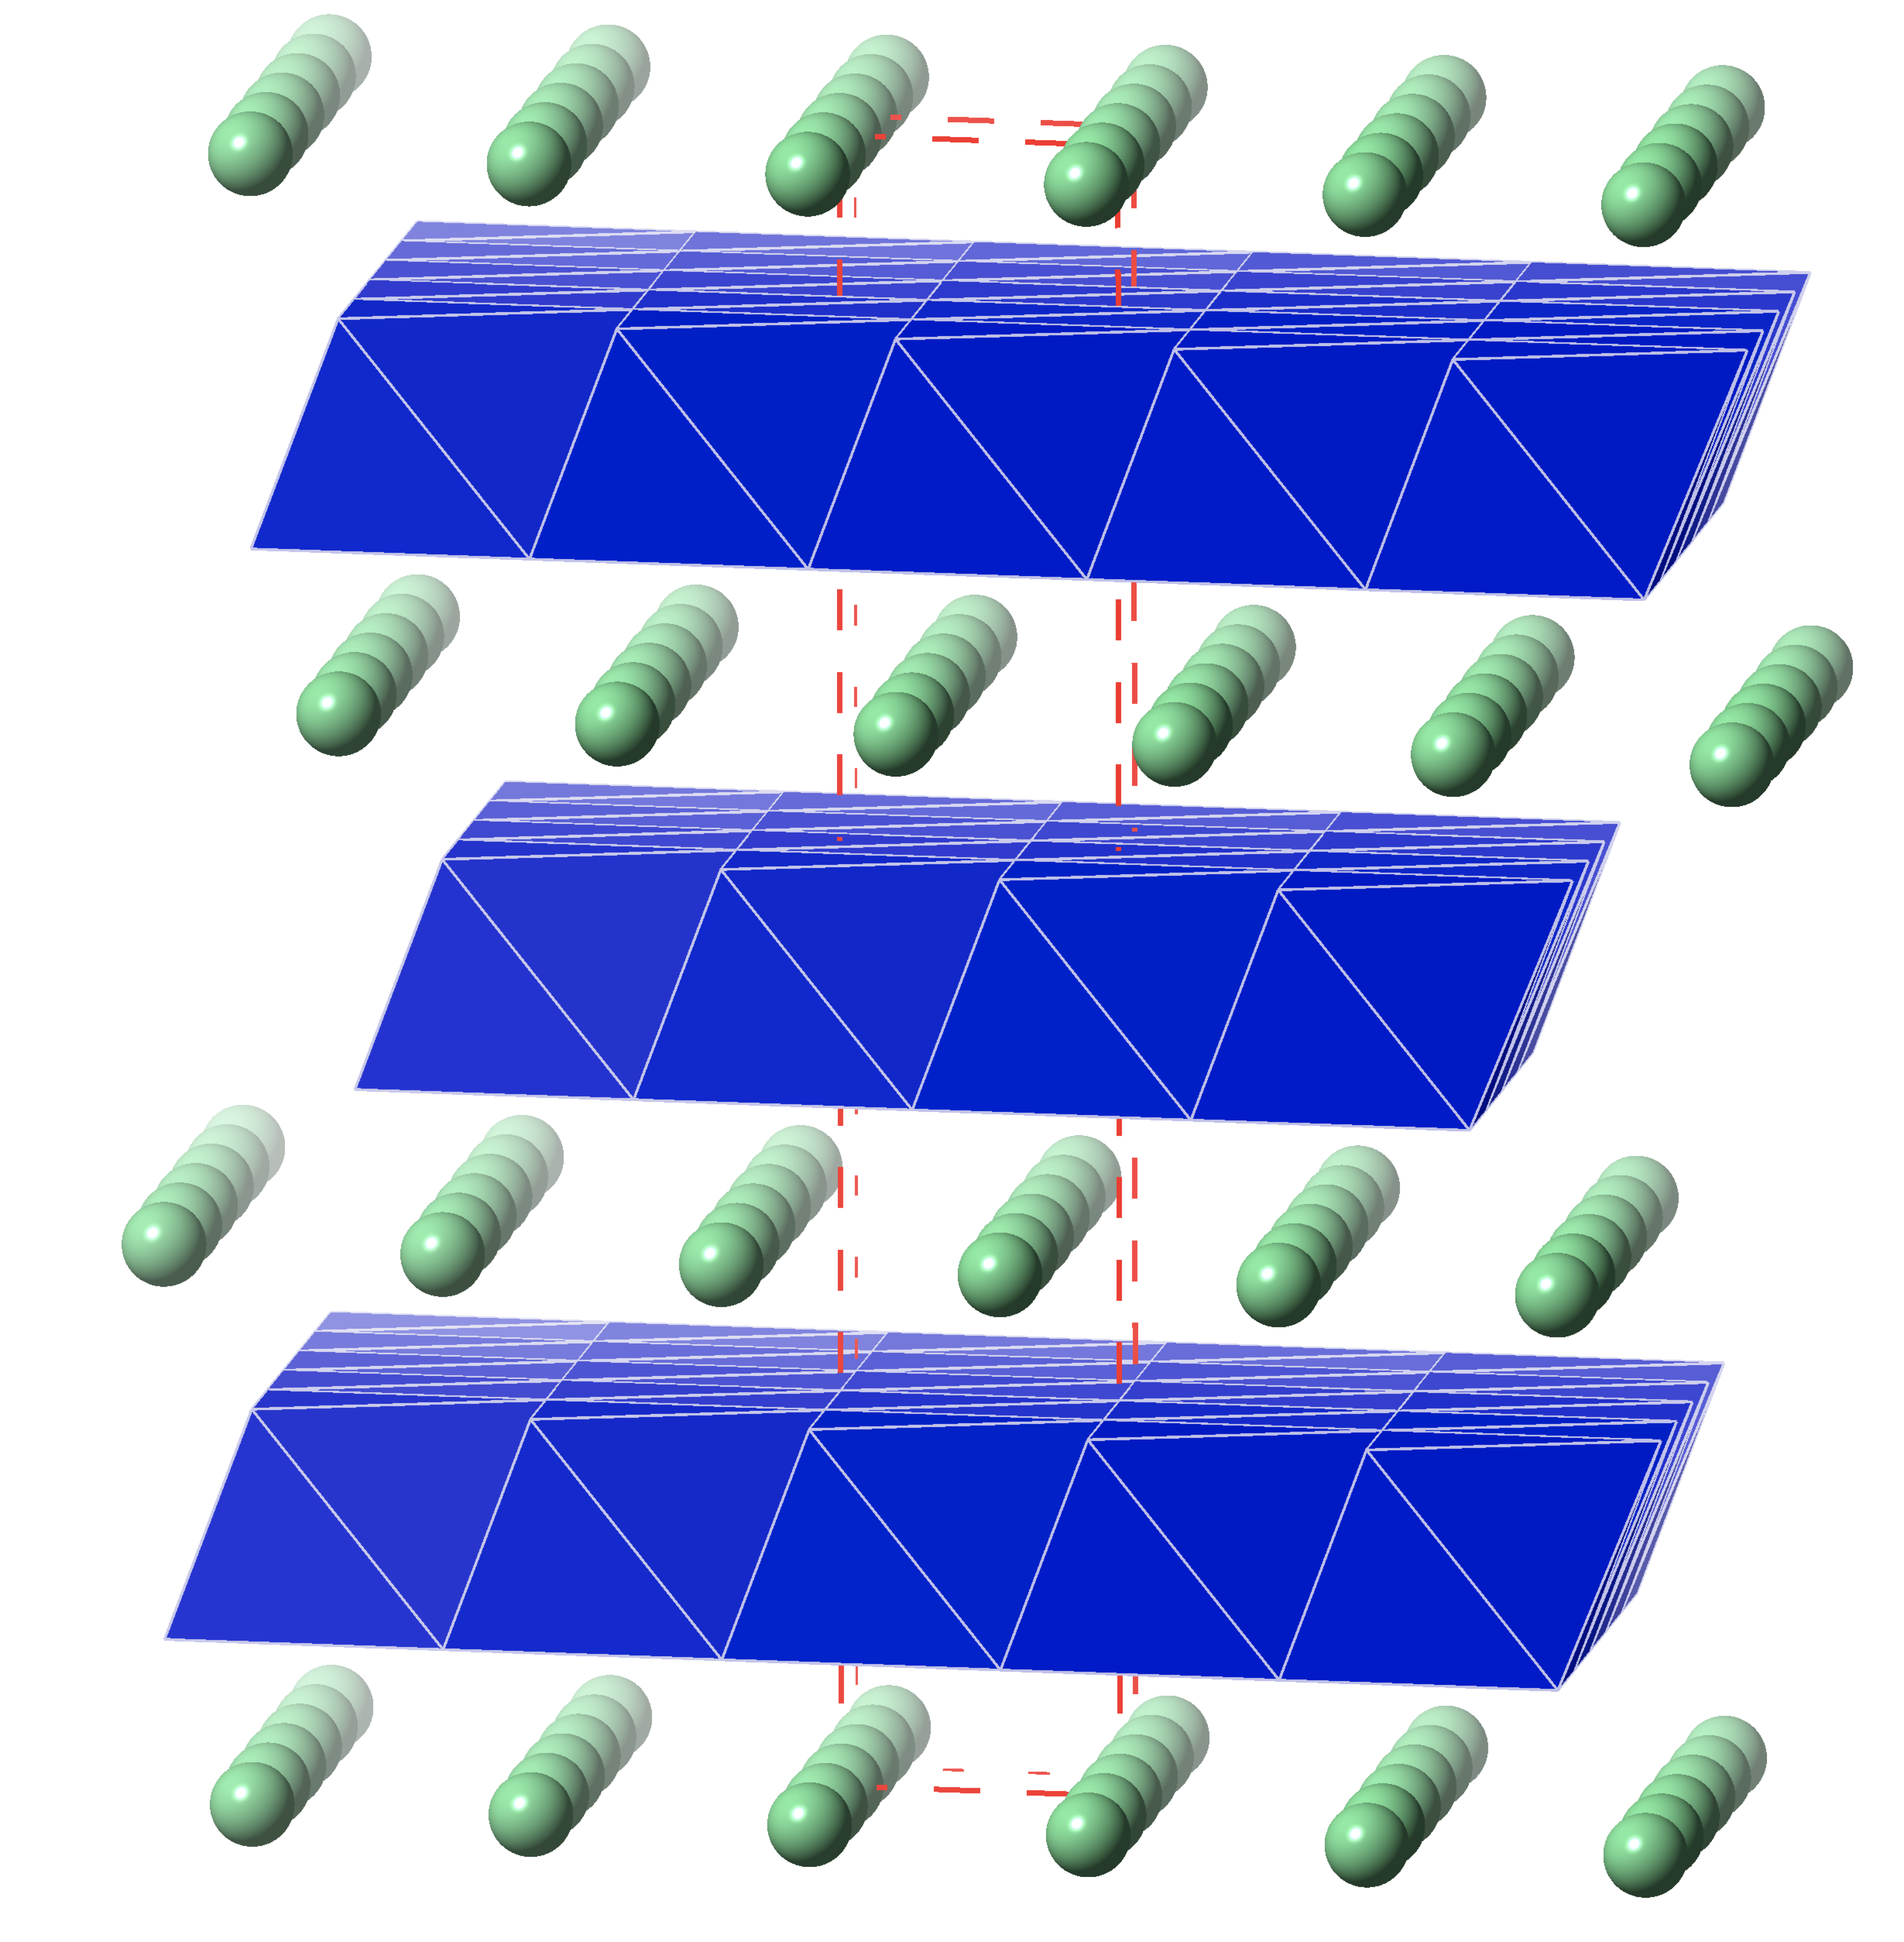
\includegraphics[height=0.6\linewidth]{figures/structures/LiCoO2}
\caption[Layered \ce{LiMO2} structure]{Layered \ce{LiMO2} structure. (\ce{Li+} ions: green; \ce{MO6} octohedra: blue)\\ }
\label{fig:LCO}
\end{figure}
\ce{LiMO2} adopt \ce{\alpha-NaFeO2} structures (Figure \ref{fig:LCO}), which is the prototype structure of \ce{AMO2} layered cathode materials.
The structure is comprised of alternating layers of \ce{[CoO2]-} and \ce{Li+} layers ($R\bar{3}M$).\cite{Islam2014}
The low migration barrier between adjacent \ce{Li+} sites within each layer leads to fast 2D ion transport through the structure.\cite{Ellis2010a}
The reaction occurring as lithium is reversibly extracted from \ce{LiMO2} cathodes can be written as:\cite{Islam2014}
\begin{equation}
\ce{Li_{1-x}MO2(s) +$x$Li+(soln) +$x$e- <=> LiMO2(s)}
\end{equation}

Different metals allow for a larger fraction of Li to be reversibly extracted, corresponding to higher energy densities.

\paragraph{\ce{LiCoO2}}
As shown in Figure \ref{fig:Goodenough}, the first commercial rechargeable Li-ion battery used a \ce{LiCoO2} (LCO) cathode (Figure \ref{fig:LCO}).
Its capacity of around \SI{150}{\milli\ampere\hour\per\gram} constituted a step change from its predecessors when it was introduced in the 1990's, and it remains prevalent in commercial applications today, particularly in portable electronics.\cite{Goodenough2013}

That said, a number of issues exist with LCO cathodes.
Firstly, the delithiation of the cathode is only reversible up to 50 \% removal of the total Li, thus around half of the theoretical capacity (\SI{275}{\milli\ampere\hour\per\gram}) cannot be reversibly accessed.\cite{Rozier2015}
Additionally, there are a number of ethical, economic, and sustainability issues associated with the supply of cobalt,\cite{Mauger2017, Larcher2015} driving research into layered metal oxide chemistries using other metals:\cite{Rozier2015}

\begin{labeling}{\textbf{\ce{LiMnO2}}}
	\item [\textbf{\ce{LiNiO2}}] Despite being cheaper, more sustainable, and having a higher theoretical capacity (\SI{200}{\milli\ampere\hour\per\gram}) than \ce{LiCoO2}, the low thermal stability of lithium nickel oxide cathodes in the presence of organic electrolytes poses a significant safety risk, making it unsuitable for commercial applications.
	Furthermore, it is not easily synthesised due to the formation of non-stoichiometric compounds arising from the spontaneous reduction of \ce{Ni^3+} to  \ce{Ni^2+}, resulting in \ce{Ni^2+} ions on \ce{Li+} sites.\cite{Das2017}
	\item [\textbf{\ce{LiMnO2}}] The similarity of the ionic radii of high-spin \ce{Mn^3+} (\SI{0.65}{\angstrom}) and \ce{Li+} (\SI{0.76}{\angstrom}) prevents the formation of stable layered \ce{LiMnO2}.\cite{Rozier2015,Rossen1992}
	While metastable \ce{LiMnO2} can be synthesised, the more stable \ce{LiMn2O4} forms upon cycling, giving poor electrochemical performance.
\end{labeling}

\newpage
\subsection{Mixed-metal layered \ce{LiMO2}}
A strategy to incorporate some of the benefits of \ce{LiNiO2}, whilst overcoming the stability and synthesis issues which have prevented its practical use is the partial substitution of Ni for other metals.\cite{Rozier2015}
Binary and ternary \ce{LiMO2} have been extensively studied, yielding compounds which have enjoyed commercial success.
Each of the below compounds have the same layered structure as \ce{LiCoO2} shown in Figure \ref{fig:LCO}, with the occupancy of each metal site determined by the stoichiometry of the mixed-compounds, and any relevant cation ordering effects.

\paragraph{\ce{Li[Ni_{1-y-z}Co_yAl_z]O2} (NCA)}
The issues with \ce{LiNiO2} arise due to the instability of \ce{Ni^3+} at elevated temperatures, and the similar ionic radii of \ce{Ni^2+} and \ce{Li+} causing migration of \ce{Ni} into the \ce{Li} layers.\cite{Das2017}
\ce{Li[Ni_{1-y-z}Co_yAl_z]O2} (NCA) type cathodes overcome these issues through the partial substitution of \ce{Ni^3+} with \ce{Co^3+} and \ce{Al^3+}:
\begin{labeling}{\textbf{\ce{Co^3+}}}
\item [\textbf{\ce{Co^3+}}] The addition of \ce{Co^3+} stabilises \ce{Ni^3+} at elevated temperatures, minimising the formation of \ce{Ni^2+}.
The similar ionic radii of \ce{Co^3+} (\SI{0.545}{\angstrom}) and \ce{Ni^3+} (\SI{0.56}{\angstrom}) allows the formation of \ce{Li(Ni,Co)O2} solid solutions.\cite{Rozier2015}
The large difference in ionic radii of these species with \ce{Li+} leads to M/Li ordering and stable layered oxides.

\item [\textbf{\ce{Al^3+}}] \ce{Al^3+} cations occupy M sites in the \ce{MO2} layers.
The stronger \ce{Al-O} bonds (relative to \ce{Co-O} and \ce{Ni-O}) serve to stabilise the cathode structure, enhancing its cycling performance and stability at high voltages.
This also enhances thermal stability, overcoming a significant barrier to the use of \ce{LiNiO2}.
As \ce{Al} is electrochemically inert, its inclusion is detrimental to the overall capacity of the cathode.
\end{labeling}

The drawbacks of including expensive Co, and inert Al are outweighed by the benefits offered by a viable layered nickel oxide cathode.
As such, \ce{LiNi_{0.8}Co_{0.15}Al_{0.05}O2} has enjoyed wide commercial success in EV applications (Tesla) with a high discharge capacity (\SI{200}{\milli\ampere\hour\per\gram}) compared to LCO.
\cite{Nitta2015}



\newpage

\begin{figure}
\centering
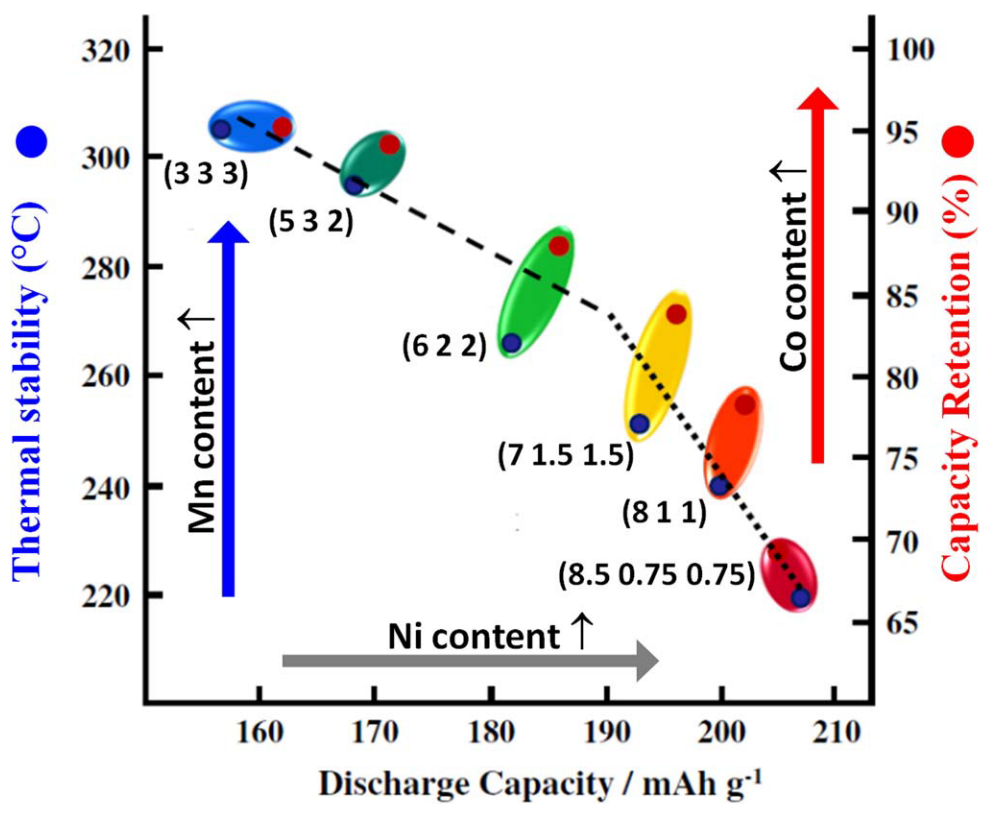
\includegraphics[width=0.5\linewidth]{figures/static/NMC_composition}

\caption[Key properties of NMC as a function of metals ratio]{Key properties of NMC as a function of metals ratio.\cite{Rozier2015, Noh2013}} 
\label{fig:NMCcomp}
\end{figure}

\paragraph{\ce{Li[Ni_{1-y-z}Mn_yCo_z]O2} (NMC)}
Initially overlooked as a poor cathode candidate when it was first reported in 1992,\cite{Rossen1992} \ce{Li[Ni_{1-x}Mn_x]O2} cathodes were revisited and expanded on in the early 2000's.\cite{Lu2001,Yabuuchi2008, Venkatraman2004}.
Whilst high temperature synthesis overcame issues associated with cation distribution,\cite{Hinuma2007} the tendency for the Ni and Mn to be in 2+ and 4+ oxidation states respectively gave rise to the same issues seen in \ce{LiNiO2}, namely \ce{Ni^2+} in the Li layer.
This meant that the high capacities observed \SI{200}{\milli\ampere\hour\per\gram} in \ce{Li[Ni_{0.5}Mn_{0.5}]O2} were only accessible at low discharge rates due to inhibited Li migration, limiting the practicality of this material as a cathode.

As with LCA, the partial substitution of \ce{Ni} for \ce{Co} limited the formation of \ce{Ni^2+} in the Li layer, leading to the \ce{Li[Ni_{1-y-z}Mn_yCo_z]O2} (NMC) class of materials.
\ce{Li[Ni_{1/3}Mn_{1/3}Co_{1/3}]O2} (NMC-111, named for the Ni:Mn:Co ratio) is currently commercialised with a practical reversible capacity of \SI{180}{\milli\ampere\hour\per\gram}.

Figure \ref{fig:NMCcomp} shows the discharge capacity, thermal stability, and capacity retention for various NMC compositions.
Broadly speaking, the discharge capacity of the material is improved by increased Ni content, the thermal stability improved by increased Mn content, and the capacity retention improves with increasing Co content.
As such, research efforts focusing on retaining high capacity retention and thermal stabilities at higher Ni concentrations are plentiful.
One promising strategy to achieve this is the formation of hierarchical cathode particles, with high capacity Ni-rich cores and stable Mn-rich shells. \cite{Zhou2018}
\newpage
\begin{figure}
\centering
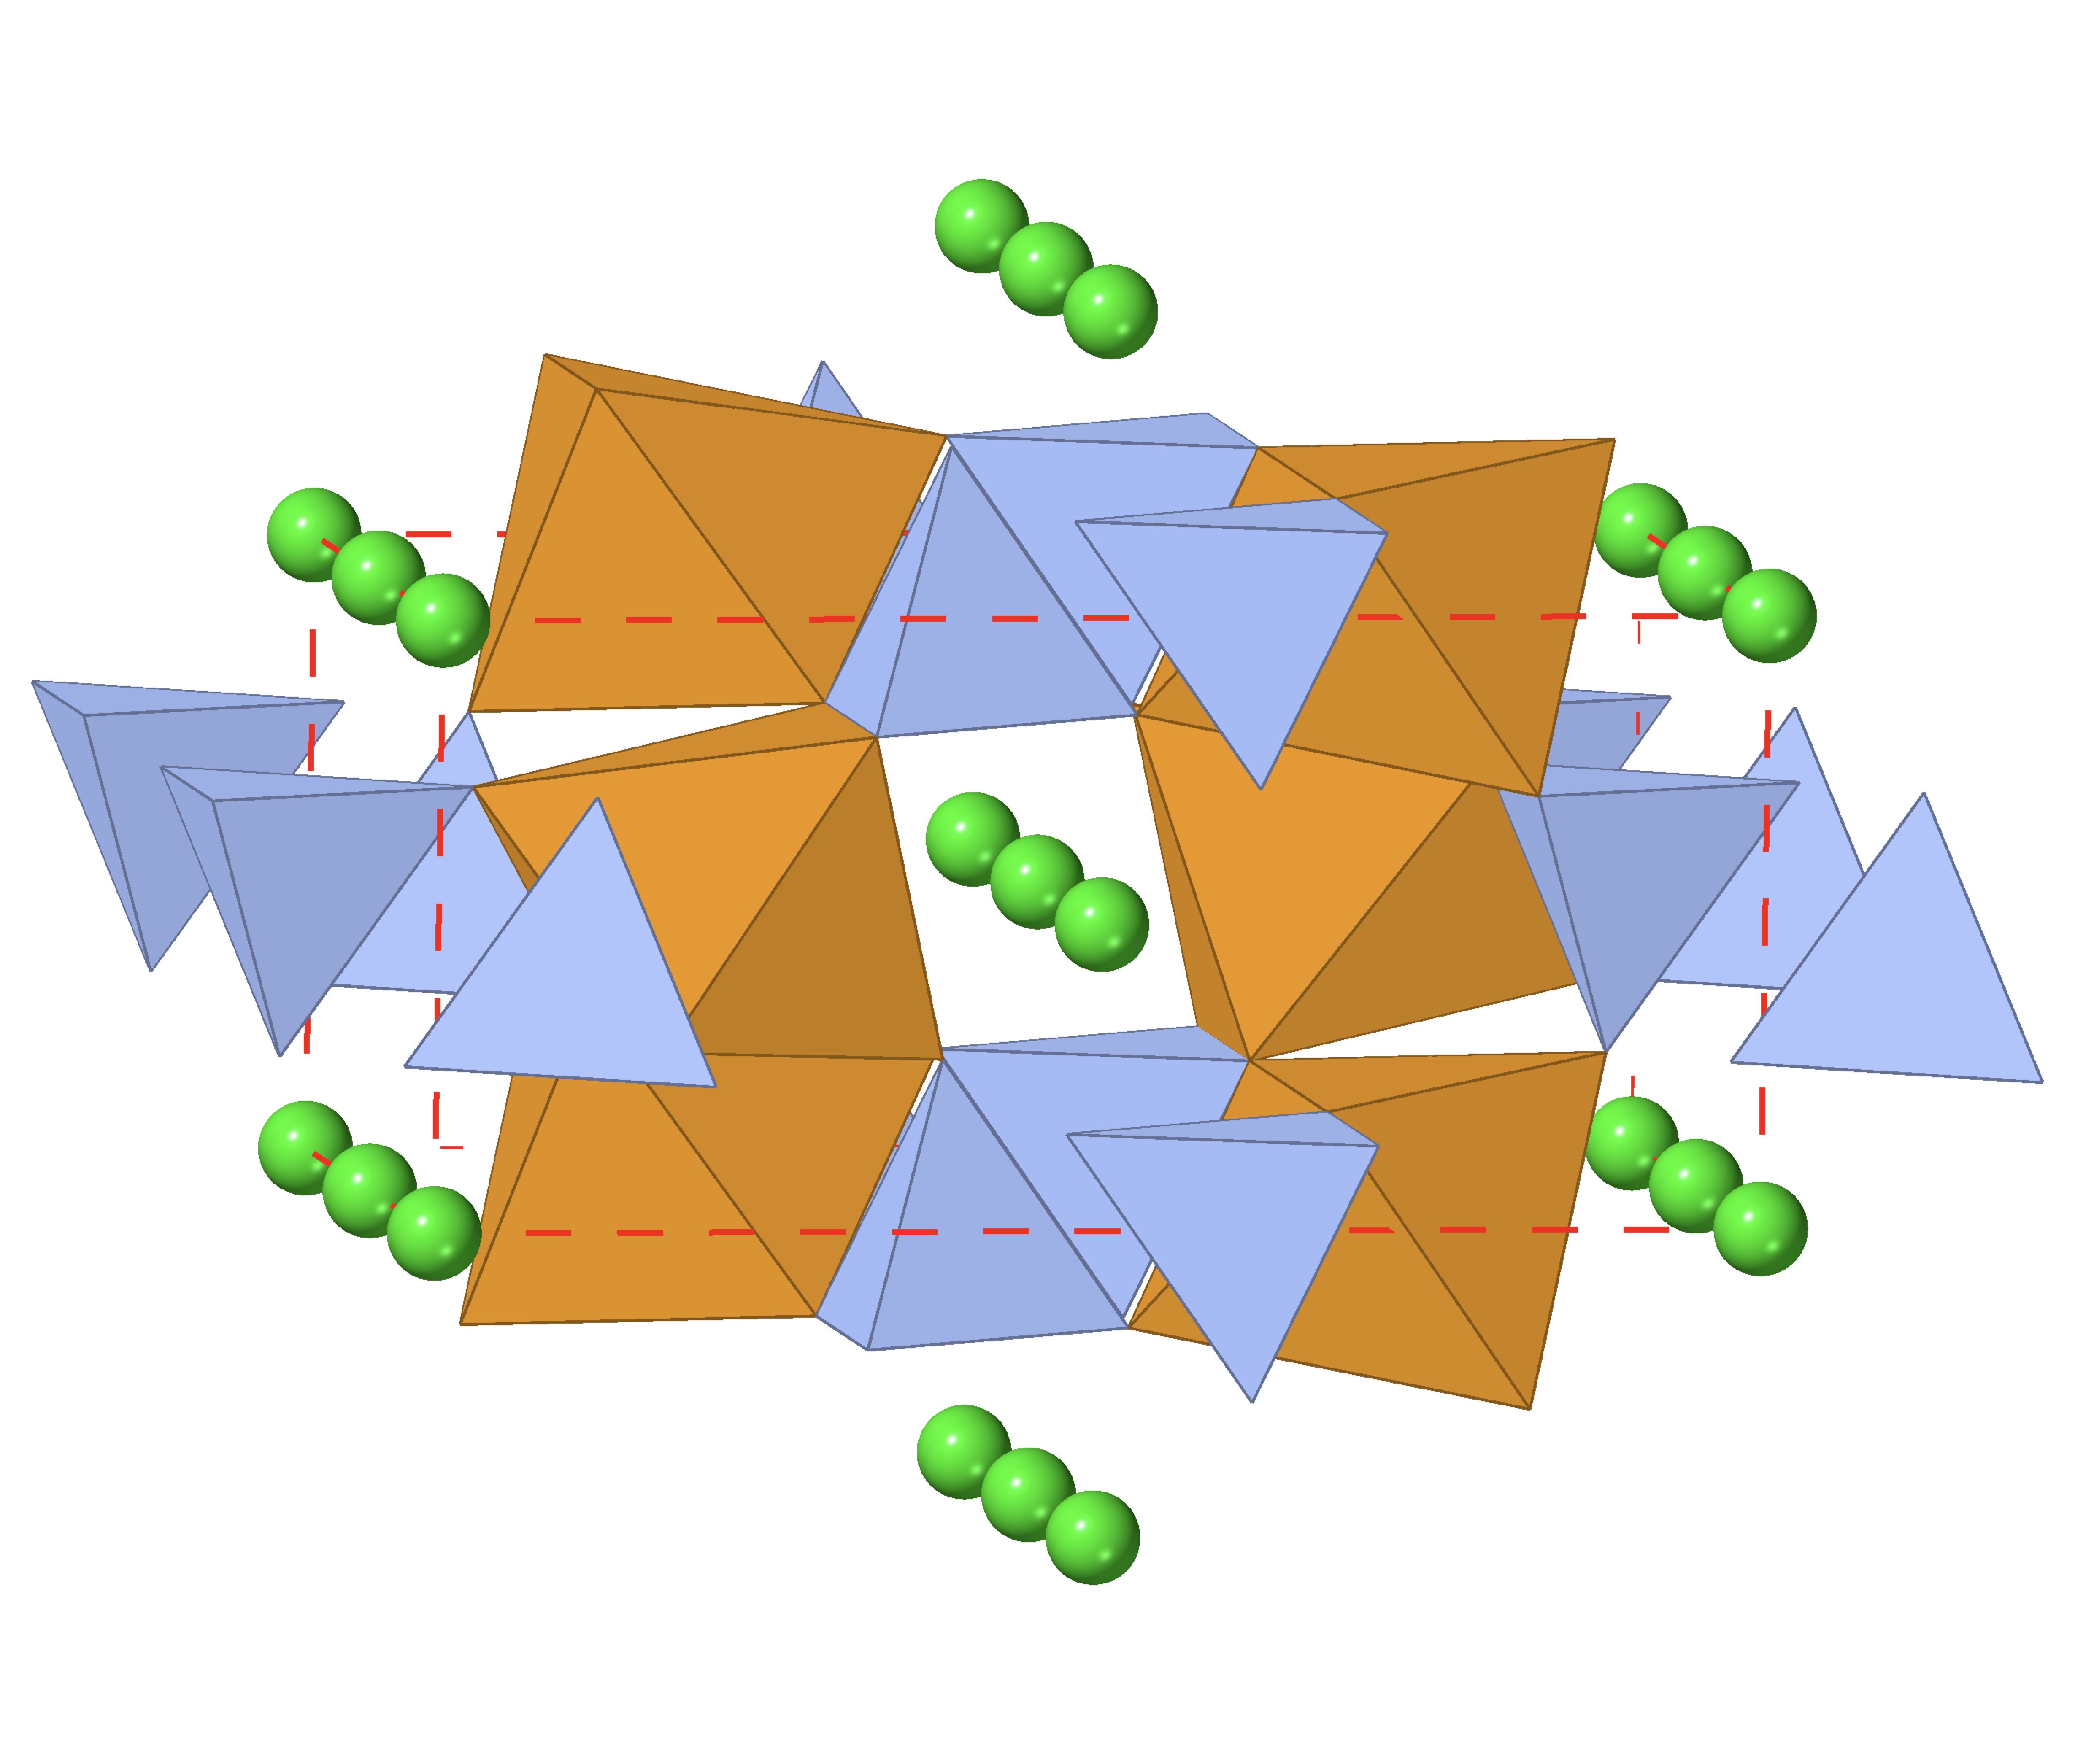
\includegraphics[width=0.6\linewidth]{figures/structures/LiFePO4}

\caption[Olivine-type \ce{LiFePO4}]{Olivine-type \ce{LiFePO4}.  \ce{Li} ions: green; \ce{Fe-O} octohedra: orange; \ce{PO4} tetrahedra: blue.} 
\label{fig:polyanion}
\end{figure}

\subsection{Polyanionic cathodes}
Polyanionic cathodes, derived from the substitution of oxide sites in layered oxides with \ce{(XO_4)^n-}/\ce{(X_mO_{3m+1})^n-} polyanions (X = S, P, Si, As, Mo, W),\cite{Gong2011a} remain of significant research interest.
The strong covalent bonding between these polyanions and \ce{MO_$x$} polyhedra leads to high thermal stability, making these materials suitable for safety critical applications.\cite{Nitta2015}

Goodenough et al.\cite{Padhi1997} initially presented the archetypal polyanionic cathode in 1997, olivine \ce{LiFePO4} (Figure \ref{fig:polyanion}), which remains the only commercialised cathode of this class.
An inductive effect from the \ce{(PO4)^3-} raises the redox potential of the \ce{Fe} centre, yielding a relatively high \ce{Fe^3+/Fe^2+} redox potential of \SI{3.5}{\volt} versus \ce{Li/Li+}, making it suitable for practical applications.
Indeed, this material is commonly used in high power situations, such as power tool applications.
The use of Fe rather than Co significantly reduces material costs, and increases the environmental credentials of this material.

The 1D migration channels\cite{Islam2014} somewhat hinder advancements via metal substitution of this cathode, as those metals with moderate \ce{Li/M} antisite defect concentrations suffer from reduced performance arising due to channel blocking.\cite{Fisher2008b}

\newpage
\begin{figure}
\centering
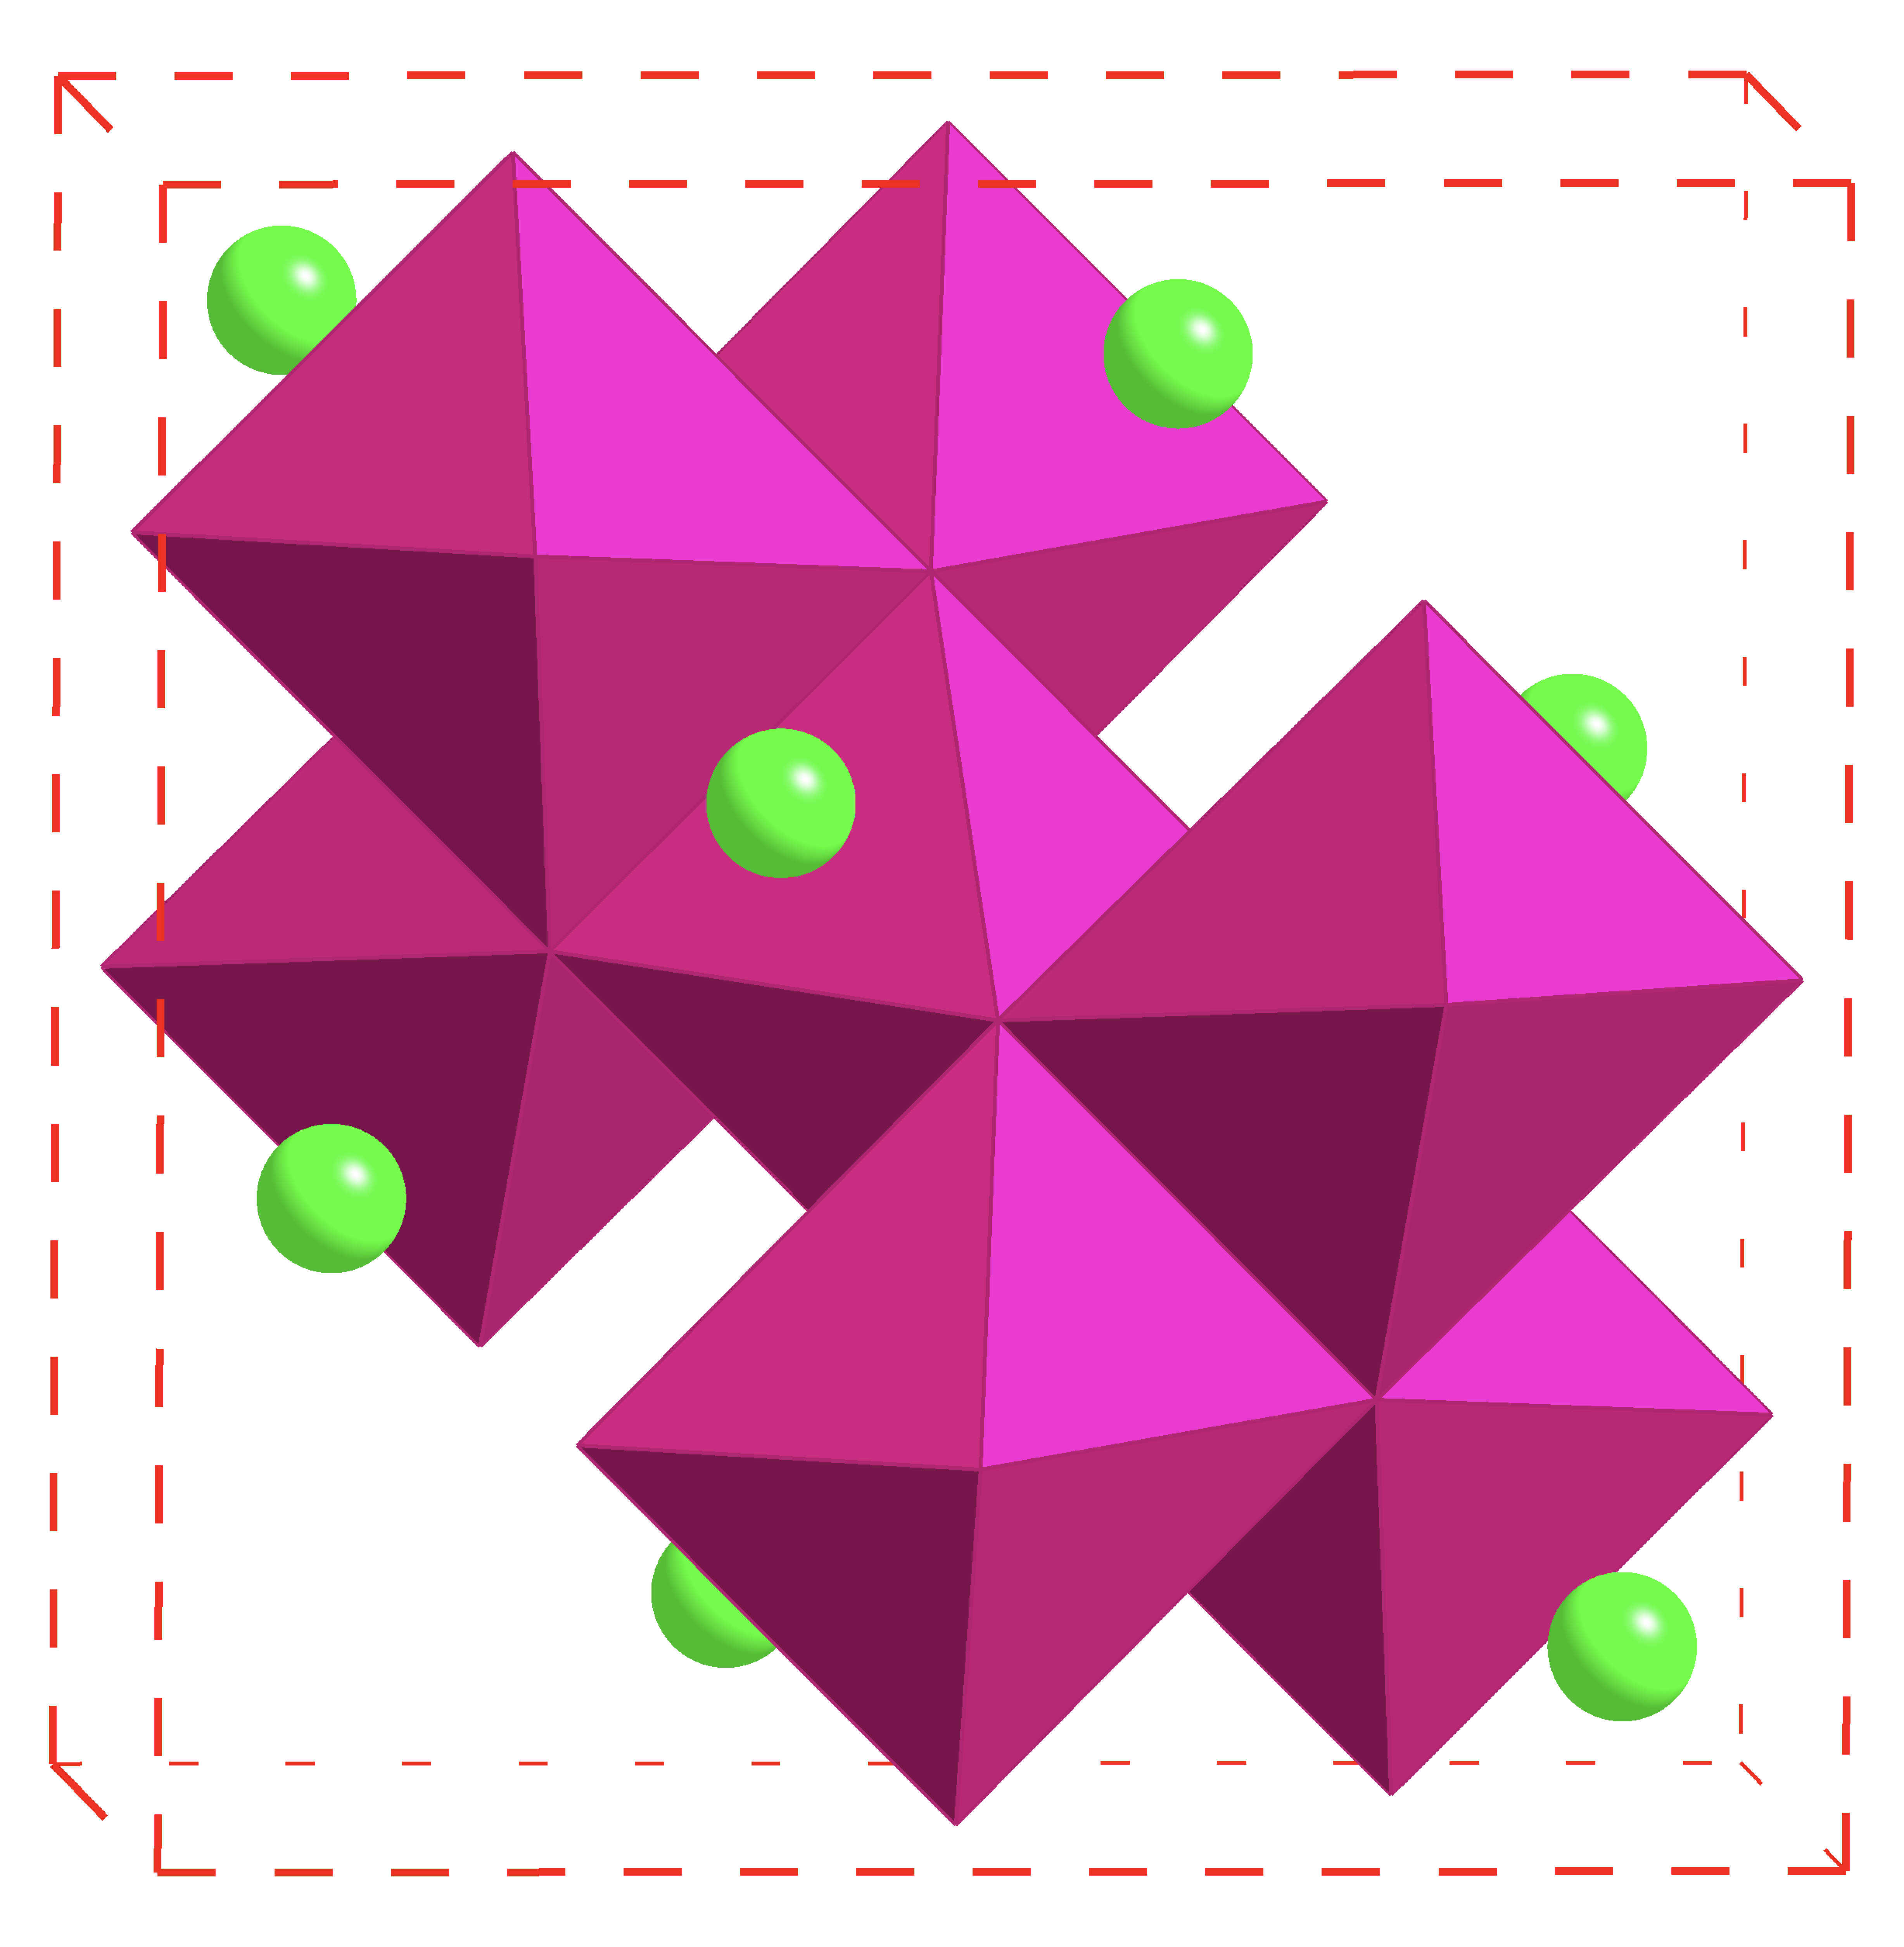
\includegraphics[width=0.7\linewidth]{figures/structures/LiMn2O4}
\caption[Cubic \ce{LiMn2O4} spinel]{Cubic \ce{LiMn2O4} spinel. \ce{Li} ions: green; \ce{MnO6} octohedra: pink.} 
\label{fig:spinel}
\end{figure}

\subsection{\ce{LiMn2O4} spinel (LMO)}
Despite its relatively low capacities (\SI{140}{\milli\ampere\hour\per\gram}), \ce{LiMn2O4} spinel (LMO) has found some commercial success in applications requiring high discharge rates.
Low internal resistance, arising from the 3 dimensional ion conduction pathways, allow for rapid cycling at high currents.

Whilst pure LMO batteries are uncommon, they are commonly coupled with NMC cathodes in EV applications, with the NMC component providing larger capacities, and the LMO component enabling for short periods of high current discharge, as required during rapid acceleration.
This strategy of combining battery chemistries is used in a number of production vehicles including the Nissan Leaf.\cite{Schmuch2018, Blomgren2017}
These cathodes also offer good thermal stability, but have a poor lifespan.
As such, there is interest in phasing out this material to extend the life of new electric vehicles.
\newpage
\section{Li-rich cathodes}
A limitation of the layered oxide materials discussed thus far is the limited extent to which delithiation can reversibly occur.
Even were a means of stabilising these cathodes in a fully delithiated state devised, the theoretical maximum capacities of conventional layered oxide cathodes may be insufficient for future automotive applications.

Li-rich cathodes seek to increase the capacity of conventional \ce{LiMO2} materials by substitution of some portion of \ce{M^3+} for \ce{Li^+}.
The term ``Li-rich'' derives then from the excess of Li relative to transition metals in the cathode:
\begin{equation}
	\frac{[\textrm{Li}]}{[\textrm{TM}]} > 1
\end{equation}

Whilst this does yield higher theoretical capacities due to the increased fraction of Li in the structure, this change also has a potentially negative impact on the electrochemical performance of the cathode:
\begin{labeling}{\textbf{Redox well}}
	\item [\textbf{Stability}] The removal of \ce{M} reduces the number of stabilising \ce{M-O} bonds.
	This reduces the thermal stability and cycle life of the cathodes.
	\item [\textbf{Redox well}] Transition metal species serve to charge compensate the extraction of \ce{Li+} from the cathode.
	Reduced transition metal availability requires other charge compensation mechanisms to allow full extraction of Li.
	\end{labeling}

As Li extraction in excess of one Li per transition metal species has been observed in many Li-rich cathodes, other charge compensation mechanisms must exist.
These mechanisms have been the area of much research, and despite extensive literature on the topic,\cite{Rozier2015,Csernica2019, Li2018a, Seo2016} it remains an area of active debate.
Of particular interest is the O-redox mechanism which has been demonstrated in many systems.\cite{Li2018a}

Whilst many Li-rich materials have been shown to be oxygen-redox-active, they generally exhibit undesirable characteristics including voltage fade, hysteresis, and O loss.\cite{Csernica2019}
The factors which impact these phenomenon have been extensively studied but remain an active and unresolved area of research.\cite{Rozier2015,Csernica2019, Li2018a, Seo2016}
\newpage
\subsection{\ce{Li2MnO3}}
\ce{Li2MnO3}, being an end member of the Li-rich layered oxide cathodes, is one of the most widely studied Li-rich materials.
It exhibits a O3-type monoclinic structure, with an ordered (honeycomb) distribution of \ce{Li+/Mn^4+} ions in the mixed \ce{[Li_{1/3}Mn_{2/3}]O2} layer.\cite{Rozier2015}

Initially thought to be electrochemically inactive due to the already fully oxidised \ce{Mn^4+}, \ce{Li2MnO3} was later shown to  demonstrate a huge theoretical capacity of \SI{285}{\milli\ampere\hour\per\gram}.\cite{Kuganathan2019a}
The electrochemical activity was attributed to a partial loss of \ce{Li2O}, leading to the formation of \ce{Li2MnO3} domains in a \ce{LiMnO2} matrix on partial delithiation.

The use of \ce{Mn} offers huge environmental and economic benefits versus \ce{Co} containing cathodes.
Unfortunately, its poor structural stability during cycling and low electrical conductivity render its use in any practical application infeasible.
It does however provide a relatively simple reference material for study, to allow a better understanding of more complex Li-rich layered oxides.





\begin{figure}
\centering
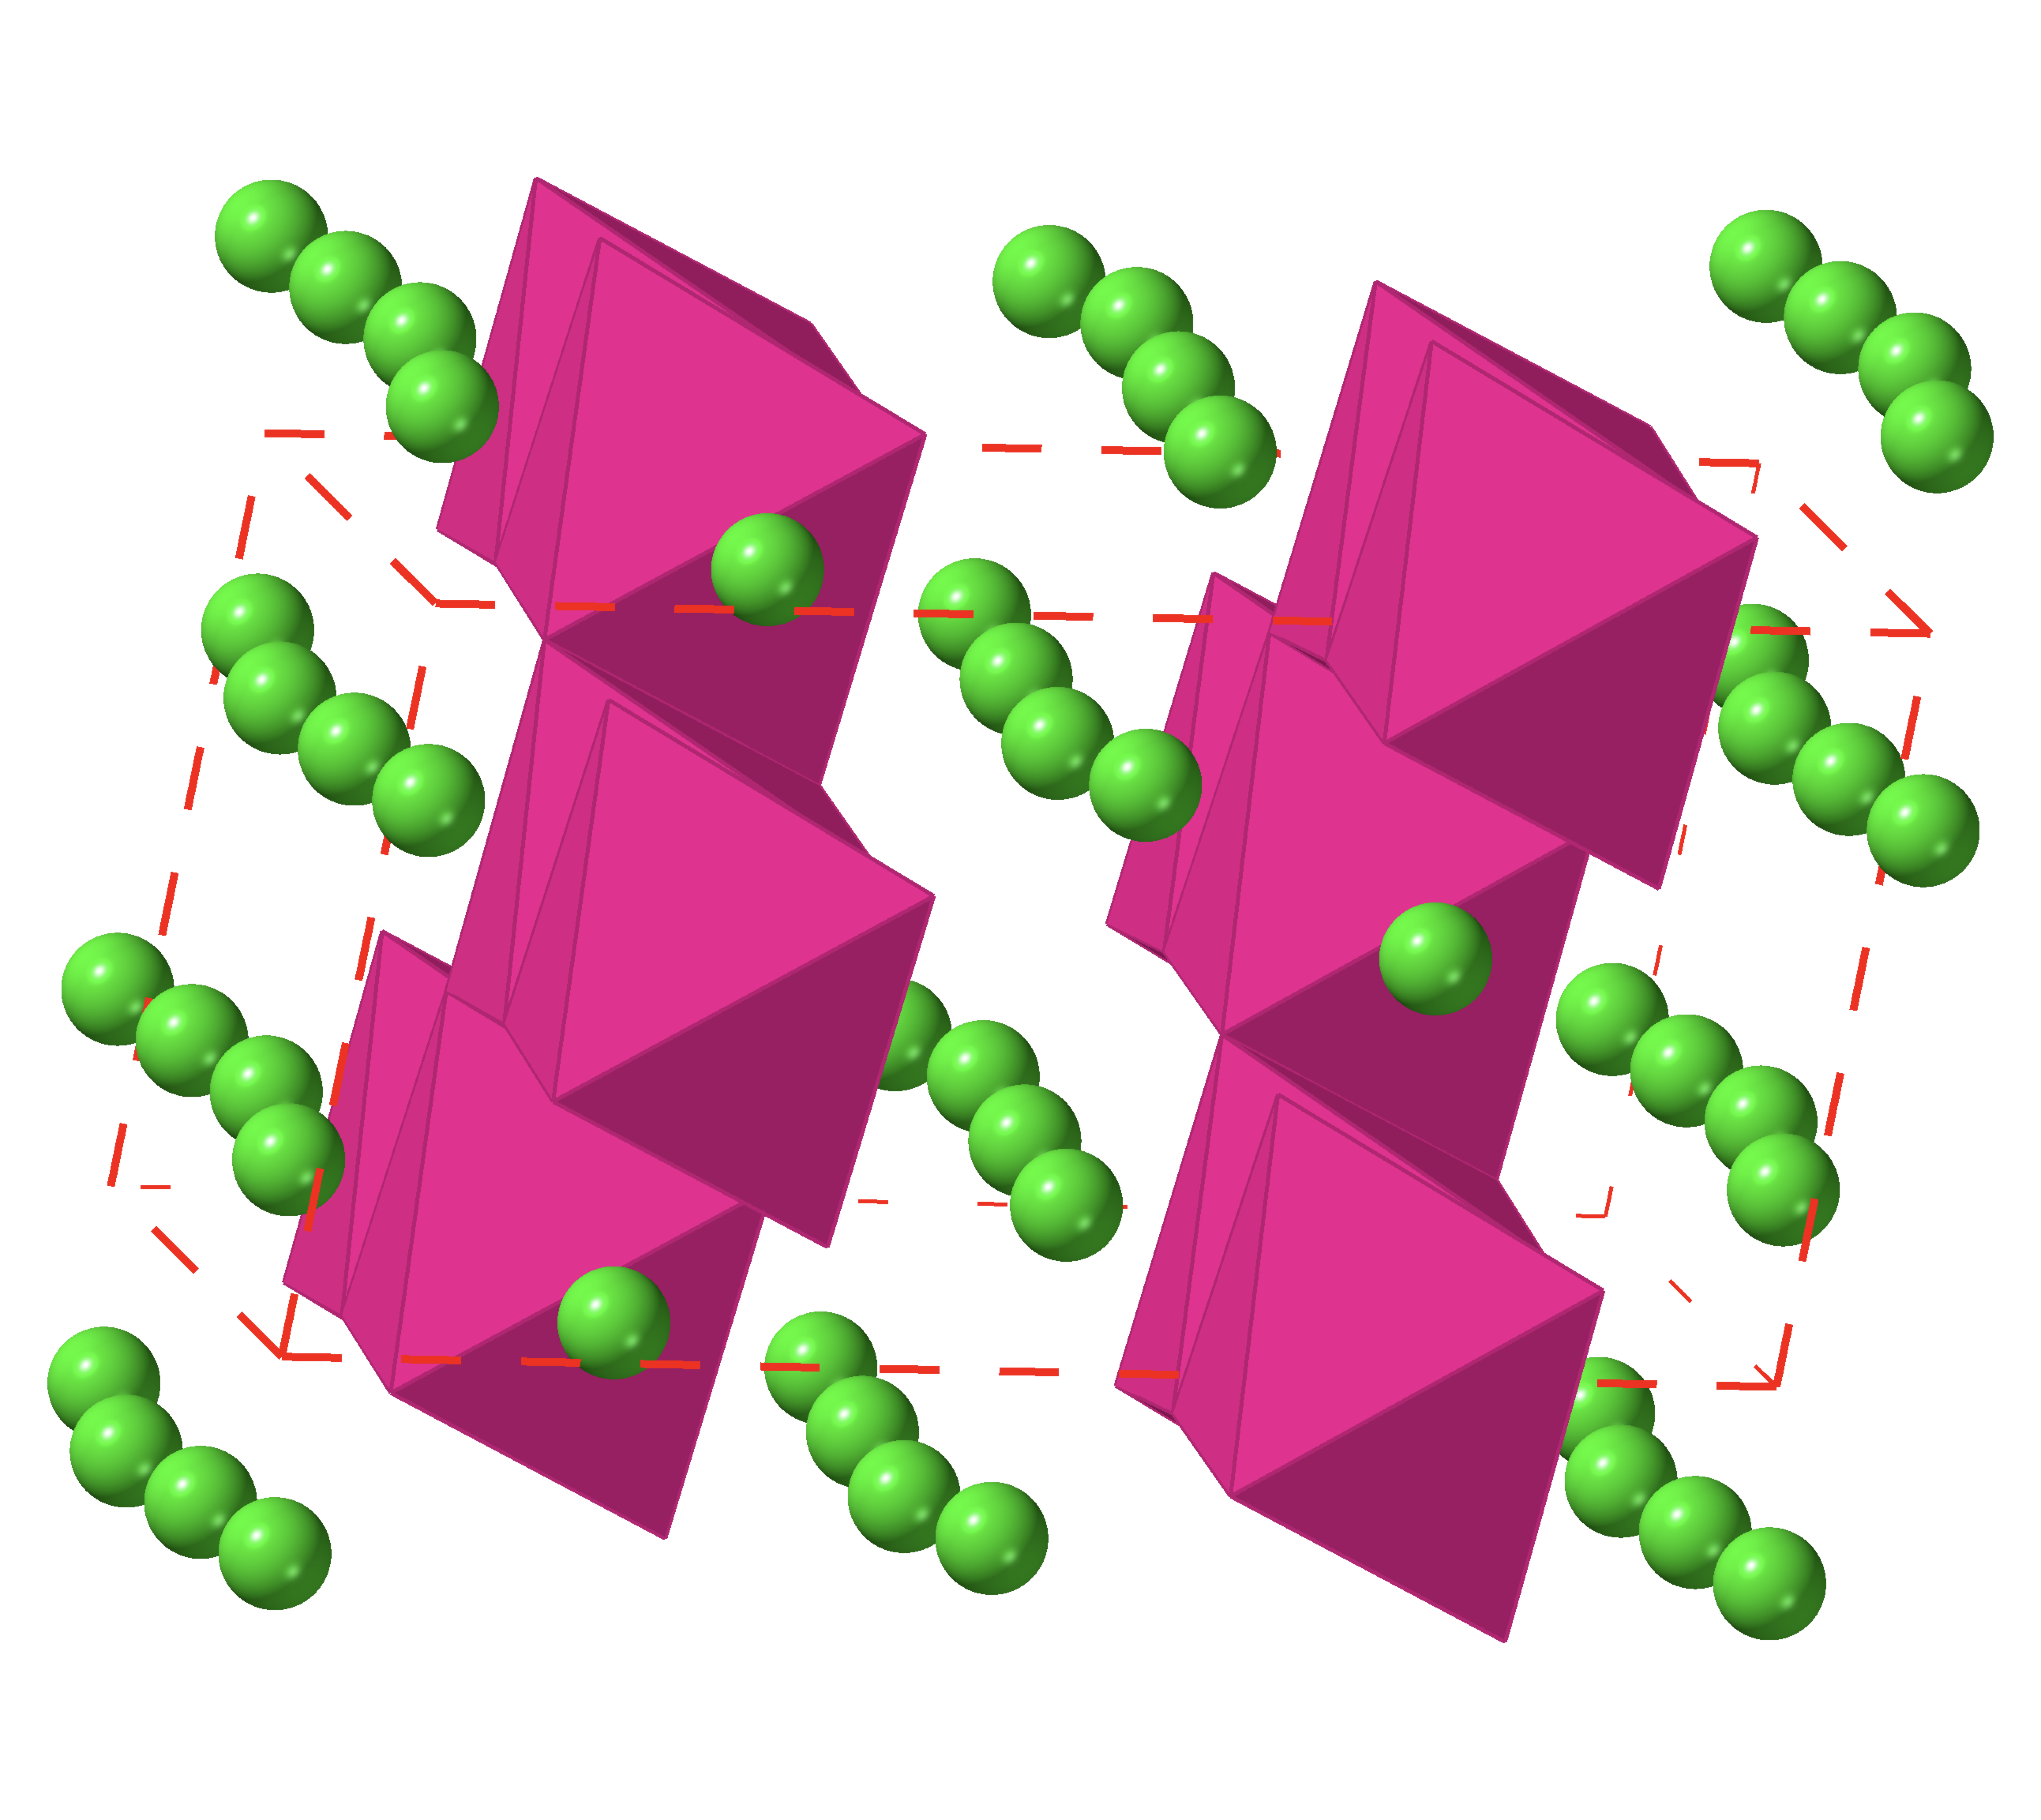
\includegraphics[width=0.6\linewidth]{figures/structures/Li2MnO3}
\caption[\ce{Li2MnO3}]{Layered \ce{Li2MnO3}. \ce{Li} ions: green; \ce{MnO6} octohedra: pink.} 
\label{fig:Li2MnO3}
\end{figure}





\newpage
\subsection{Li-rich NMC}
\begin{figure}
\centering
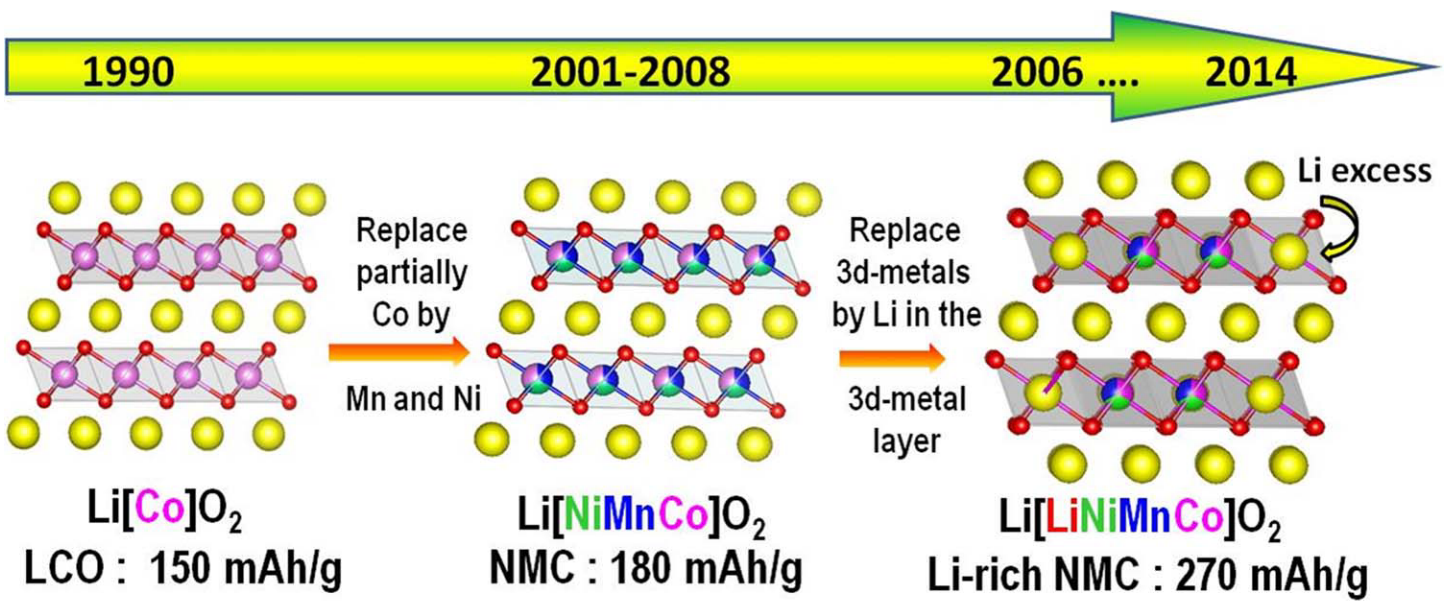
\includegraphics[width=\linewidth]{figures/structures/tarasconNMC}
\caption[Evolution of Li-rich NMC from LCO.]{Evolution of Li-rich NMC from LCO.\cite{Rozier2015}} 
\label{fig:tarasconNMC}
\end{figure}

Li-rich NMC, shown schematically in Figure \ref{fig:tarasconNMC}, is NMC in which some metal species have been exchanged fo Li.
As with the \ce{LiMO2} cathodes, the rich chemistry associated with the presence of multiple metal species offers a wide range of compositions and provides scope to overcome some of the issues associated with the current state of the art Li-rich cathodes, such as voltage fade and O-loss.
Surface coatings have been proposed as a means of extending the lifetime of Li-Rich NMC cathodes, by preventing side reactions with the electrolyte and limiting the formation of non-conductive species which harm electrochemical performance.
Whilst an undeniably useful avenue of research, the additional processing steps may make the implementation of this at a commercial scale infeasible.
Furthermore, the absence of a fundamental understanding of the mechanisms giving rise to these detrimental properties will inevitably hinder progress.
As the exact origin of these phenomenon is not widely agreed upon, and may indeed change between systems, much of the research surrounding Li-rich NMC has been in attempting to better understand the fundamental phenomenon which give rise to these undesirable properties.


\newpage
\subsection{Li-rich disordered rocksalts}
Conventional cathode materials tend to have ordered structures, as the presence of distinct transition metal sites and Li sites/diffusion pathways provides stability upon cycling.
The lack of intermixing of Li and transition metal species is vital to ensure good Li-ion mobility and prevent detriment to electrochemical performance.
Ceder \textit{et al.}\cite{Casimir2014} proposed however, that the ``ordering paradigm'' adopted by the battery community led to a number of viable cathode candidates being overlooked.
By percolation theory, so long as the ratio of Li:TM sites is above some critical concentration, a network of low-energy pathways should exist, allowing mobility and extraction to occur.\cite{Urban2014}

Of particular interest in this work are two disordered rocksalt structures:

\begin{labeling}{\textbf{\ce{Li2MnO2F}}}
\item [\textbf{\ce{Li4Mn2O5}}] First presented in 2015 by Freire \textit{et al.},\cite{Freire2016} this material demonstrates a huge specific capacity of \SI{355}{\milli\ampere\hour\per\gram}.
Diaz-Lopez \textit{et al.}\cite{Diaz-Lopez2018} characterised the material, demonstrating that a \ce{MnO} rocksalt structure with high \ce{Li/Mn} disorder at cationic sites, and 1/\nth{6} O vacancies at the anionic site provided good agreement with synchrotron and powder diffraction data.
Yao \textit{et al.}\cite{Diaz-Lopez2017}, and later Bhattacharya \textit{et al.}, used these findings as a basis for a DFT study.
These studies identified a number of ordered structures which were of a lower energy than quasi-disordered structures.

\item [\textbf{\ce{Li2MnO2F}}] Initially presented in 2018 by Bruce \textit{et al.},\cite{House2018} \ce{Li2MnO2F} also exhibits disorder on both the cation and anion sites.
With a discharge capacity of \SI{280}{\milli\ampere\hour\per\gram}, half of which arises from O-redox, the material is both an interesting candidate to better understand the anion redox processes exhibited in other Li-rich cathodes, and an excellent cathode candidate itself.
Furthermore, there is little evidence of O-loss, distinguishing it from layered Li-rich cathodes.
There is currently no literature beyond the paper in which the material was initially presented. 
Dr Ryan Sharpe, in collaboration with the author, is currently preparing a manuscript pertaining to a DFT study of this material.
\end{labeling}

\section{Project aims and chronology}
Whilst both \ce{Li4Mn2O5} and \ce{Li2MnO2F} have been studied with DFT, either in literature or in preparation, there have thus far been no defect or dynamic computational studies of either material.
This information may be key to understanding the role of local ordering on electrochemical performance, and may inform future experimental work.
As such, this work contains atomistic studies of each of these materials, focusing particularly on properties of interest for battery materials.

It is worth clarifying at this point that the trivial tone in which the above problem is stated in no way correlates with the difficulty of the task!
Much of the work done in the past year has focused on methods development, as the disordered nature of these materials demands the use of interatomic potentials which are stable for a wide range of local environments.
Furthermore, random structure generation lends itself to the creation of unphysical local environments by the law of large numbers if not biased against.
Whilst readily handled in DFT, where the first principles nature of the calculations lend themselves well to handling a wide range of states, interatomic potentials are generally derived to describe a particular system.
Disordered systems, with more local environments than conventional ordered materials, give rise to a number of issues in atomistic simulations.

\ce{Li2MnO2F} was the first material studied in this project. 
The difficulties in obtaining reasonable results were attributed not to the disorder in the system, but to the lack of a suitable Mn-F potential in literature.
It was only when similar issues manifested in the \ce{Li4Mn2O5} system that the disorder was identified as the source of difficulty. 

